\clearpage
\subsection{Categories}
\label{sec:bg_cat}
As a relatively young branch of mathematics, category theory studies, in an abstract way, the properties of particular mathematical structures. It seeks to express all mathematical concepts in terms of ``object'' and ``morphisms'' independently of what they are representing. Nowadays, categories appear in most branches of mathematics and many parts of computer science. For instance, topoi, a kind of category, can even serve as a foundation for mathematics. Cartesian closed categories, as another example, can be used as a framework for describing the denotational semantics of simply typed lambda calculus, and more generally, programming languages.


%---------------------------------------------------------------------------%
%Categories
\subsubsection{Categories}
\label{sec:bg_cat_c}
The formal definition of categories is given first.
\begin{definition}[\textbf{Categories}]
\label{definition:category}
A \emph{category} $ \mathcal{C} $ consists of
\begin{myitemize}
\item a collection $ C^o $ of objects;
\item a collection $ C^m $ of morphisms (also called arrows or maps) between objects, with two maps $ dom, cod : C^m \to C^o $ which give the domain and codomain of a morphism (we write $ f : A \to B $ to denote a morphism $ f $ with $ dom(f) = A $ and $ cod(f) = B $);
\item a binary map ``$ \circ $'', called composition, mapping each pair $ f, g $ of morphisms with $ cod(f) = dom(g) $ to a morphism $ g \circ f $ such that $ dom(g \circ f) = dom(f) $ and $ cod(g \circ f) = cod(g) $;
\end{myitemize}
such that the following axioms hold:
\begin{myitemize}
\item identity: for every object $ A $, there exists a morphism $ \text{id}_A : A \to A $, called the identity morphism for $ A $, such that $ f = f \circ \text{id}_A $ and $ g = \text{id}_A \circ g $ for any morphisms $ f $ and $ g $ with $ dom(f) = cod(g) = A $;
\item associativity: $ h \circ (g \circ f) = (h \circ g) \circ f $ for every $ f: A \to B $, $ g: B \to C$, and $ h: C \to D $.
\end{myitemize}
\end{definition}

For any objects $ A $ and $ B $ in a category $ \mathcal{C} $, the collection of all morphisms $ f: A \to B $ is called a \emph{hom-set} and denoted as $ \text{Hom}_\mathcal{C}(A,B) $. A category is determined by its hom-sets.

Categorists use \emph{diagrams} to express equations. In a diagram, a morphism $ f: A \to B $ is represented as an arrow form point $ A $ to $ B $, labeled $ f $. A diagram \emph{commutes} if the composition of the morphism along any path between two fixed objects is equal. The identity and associative laws in definition \ref{definition:category} can be represented by the commutative diagrams in figure \ref{figure:cat_id_asso}.
\begin{figure}[h!]
\centering
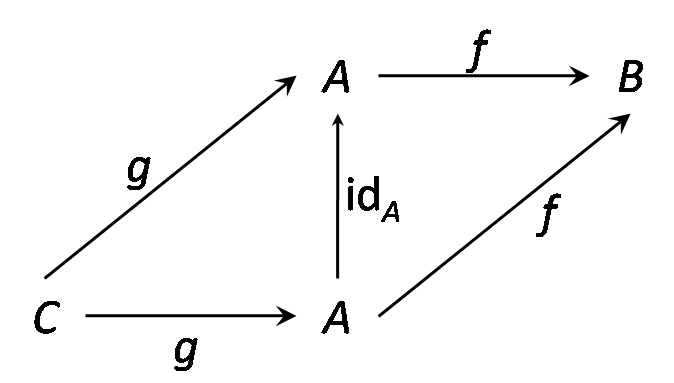
\includegraphics[scale=0.48]{./images/cat_id}
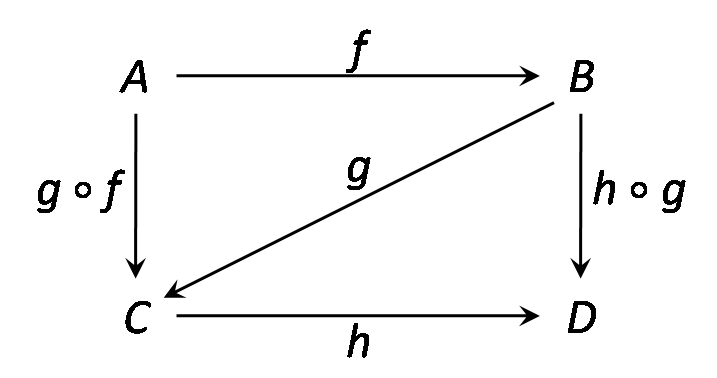
\includegraphics[scale=0.48]{./images/cat_asso}
\caption{Diagrams of identity and associativity}
\label{figure:cat_id_asso}
\end{figure}

A common example of a category is \textsc{Set} which is the category whose objects are sets and whose morphisms are functions. The identity of object $ S $ in \textsc{Set} is the identity function $ \text{id}_S : S \to S $ such that $ \text{id}_S(s) = s $ for all $ s \in S $. The composition of morphisms is the composition of functions, i.e. $ (g \circ f)(x) = g(f(x)) $. As a category, it satisfies the two category axioms:
\begin{myitemize}
\item[i)] $ f = f \circ \text{id}_A = \text{id}_B \circ f $ for every $ f: A \to B $\\
The identity follows by using the definitions of composite functions and identity functions:\\
$ (f \circ \text{id}_A)(a) = f(\text{id}_A(a)) = f(a) $ and $ (\text{id}_B \circ f)(a) = \text{id}_B(f(a)) = f(a) $.
\item[ii)] $ h \circ (g \circ f) = (h \circ g) \circ f $ for every $ f: A \to B $, $ g: B \to C$, and $ h: C \to D $\\
The associativity follows from the fact that composition of functions is associative:\\
$ (h \circ (g \circ f))(a) = h((g \circ f)(a)) = h(g(f(a))) $ and\\
$ ((h \circ g) \circ f)(a) = (h \circ g)(f(a)) = h(g(f(a))) $.
\end{myitemize}

One typical use of categories is to consider categories whose objects are sets with mathematical structure and whose morphisms are functions that preserve that structure. One of the common examples is the category \textsc{Pos} whose objects are posets and whose morphisms are monotone functions. It will be discussed later as an example of a CCC in \ref{sec:bg_cat_ccc}.


%---------------------------------------------------------------------------%
%Categorical Constructions
\subsubsection{Categorical Constructions}
\label{sec:bg_cat_cc}
There are many categorical constructions, i.e. particular objects and morphisms that satisfy a given set of axioms, which enrich the language of Category Theory. When studying constructions, one observes that all concepts are defined by their relations with other objects, and these relations are established by the existence and the equality of particular morphisms. In this dissertation, the following fundamental categorical constructions will be considered.
\\
\\
The simplest among these is the notion of initial object and its dual, terminal object.

\begin{definition}[\textbf{Initial and terminal objects}]
\label{definition:ini_ter_obj}
Let $ \mathcal{C} $ be a category. An object $ A $ in $ \mathcal{C} $ is \emph{initial} if, for any object $ B $ in $ \mathcal{C} $, there is a unique morphism from $ A $ to $ B $. An object $ A $ in $ \mathcal{C} $ is \emph{terminal} if, for any object $ B $ in $ \mathcal{C} $, there is a unique morphism from $ B $ to $ A $.
\end{definition}

In this dissertation, terminal objects are denoted as $ unit $ and, for object $ A $, the unique
morphism is denoted as $ \text{One}^A : A \to unit $.

In \textsc{Set}, the initial object is the empty set $ \emptyset $, and the unique morphism with $ \emptyset $ for its source is the empty function whose graph is empty. Any singleton set is terminal in \textsc{Set} since for any set $ S $, there is exactly one function from $ S $ to this singleton set.
\\
\\
In set theory, we can form a cartesian product of two sets and define coordinate functions for it. Then we can even form a product function of two given functions which have the same domain. This motivates a general definition of categorical products (within a category).

\begin{definition}[\textbf{Products}]
\label{definition:products}
Let $ A $ and $ B $ be objects in a category $ \mathcal{C} $. The \emph{product} of $ A $ and $ B $ is an object $ A \times B $ together with two morphisms $ \text{Proj}_1^{A,B}: A \times B \to A $ and $ \text{Proj}_2^{A,B}: A \times B \to B $, and for every object $ C $ in $ \mathcal{C} $, an operation $ \langle \cdot , \cdot \rangle : \text{Hom}(C,A) \times \text{Hom}(C,B) \to \text{Hom}(C, A \times B) $ such that for every $ f_1 : C \to A $, $ f_2 : C \to B $, and $ g : C \to A \times B $, the following equations hold:
\begin{myitemize}
\item $ \text{Proj}_i \circ \langle f_1 , f_2 \rangle = f_i $;
\item $ \langle \text{Proj}_1 \circ g , \text{Proj}_2 \circ g \rangle = g $.
\end{myitemize}
\end{definition}

Since equations in category theory can be represented by commutative diagrams, we can give another definition of categorical products based on diagrams: Let $ A $ and $ B $ be objects in a category $ \mathcal{C} $. The product of $ A $ and $ B $ is an object $ A \times B $ together with two morphisms $ \text{Proj}_1^{A,B}: A \times B \to A $ and $ \text{Proj}_2^{A,B}: A \times B \to B $, and for every object $ C $ in $ \mathcal{C} $, an operation $ \langle \cdot , \cdot \rangle : \text{Hom}(C,A) \times \text{Hom}(C,B) \to \text{Hom}(C, A \times B) $ such that for every $ f_1 : C \to A $ and $ f_2 : C \to B $, the morphism $ \langle f_1 , f_2 \rangle : C \to A \times B $ is the unique $ g $ that makes the diagram in figure \ref{figure:cat_prod} commute.
\begin{figure}[h!]
\centering
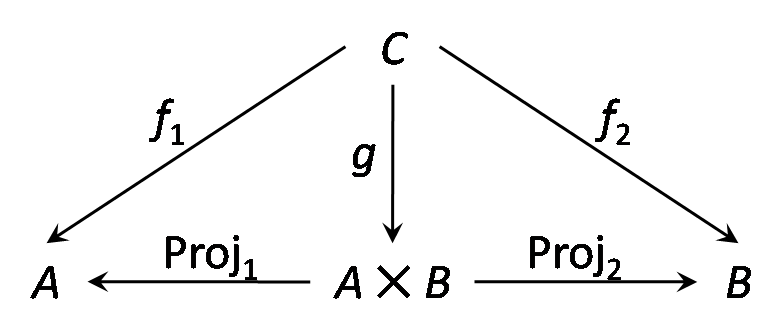
\includegraphics[scale=0.48]{./images/cat_prod}
\caption{Diagram of product $ A \times B $}
\label{figure:cat_prod}
\end{figure}

The cartesian product construction for morphisms can also be given a categorical definition. Given morphisms $ f : A \to C $ and $ g : B \to D $ the product $ f \times g : A \times B \to C \times D $ is defined by $ f \times g = \langle f \circ \text{Proj}_1^{A,B} , g \circ \text{Proj}_2^{A,B} \rangle $ whose correspondent commutative diagram is given in figure \ref{figure:cat_prod_mor}.
\begin{figure}[h!]
\centering
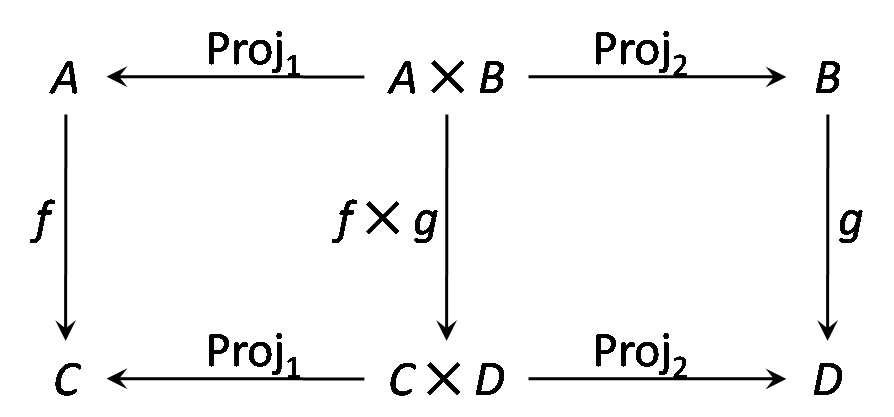
\includegraphics[scale=0.48]{./images/cat_prod_mor}
\caption{Diagram of product of morphisms}
\label{figure:cat_prod_mor}
\end{figure}

\begin{proposition}
\label{proposition:pro_of_mor}
Let $ \mathcal{C} $ be a category with products. Given $ f_1 : A \to B $, $ g_1 : B \to C $, $ f_2 : A' \to B' $ and $ g_2 : B' \to C' $, the equation $ ( g_1 \times g_2 ) \circ ( f_1 \times f_2 ) = ( g_1 \circ f_1 ) \times ( g_2 \circ f_2 ) $ holds.
\end{proposition}
\begin{proof}
\mbox\\
\\
$
\begin{array}{ll}
  & \text{Proj}_1 \circ ( ( g_1 \times g_2 ) \circ ( f_1 \times f_2 ) )\\
= & ( \text{Proj}_1 \circ ( g_1 \times g_2 ) ) \circ ( f_1 \times f_2 )\\
= & ( g_1 \circ \text{Proj}_1 ) \circ ( f_1 \times f_2 )\\
= & g_1 \circ ( \text{Proj}_1 \circ ( f_1 \times f_2 ) )\\
= & g_1 \circ ( f_1 \circ \text{Proj}_1)\\
= & ( g_1 \circ f_1 ) \circ \text{Proj}_1
\end{array}
$

Similarly, we have $ \text{Proj}_2 \circ ( ( g_1 \times g_2 ) \circ ( f_1 \times f_2 ) ) = ( g_2 \circ f_2 ) \circ \text{Proj}_2 $.

By the equation $ \langle \text{Proj}_1 \circ g , \text{Proj}_2 \circ g \rangle = g $ in definition \ref{definition:products},\\
$
\begin{array}{ll}
  & ( g_1 \times g_2 ) \circ ( f_1 \times f_2 )\\
= & \langle \text{Proj}_1 \circ ( ( g_1 \times g_2 ) \circ ( f_1 \times f_2 ) ) , \text{Proj}_2 \circ ( ( g_1 \times g_2 ) \circ ( f_1 \times f_2 ) ) \rangle \\
= & \langle ( g_1 \circ f_1 ) \circ \text{Proj}_1 , ( g_2 \circ f_2 ) \circ \text{Proj}_2 \rangle
\end{array}
$

According to the definition of products of morphisms,\\
$
\begin{array}{ll}
  & ( g_1 \circ f_1 ) \times ( g_2 \circ f_2 )\\
= & \langle ( g_1 \circ f_1 ) \circ \text{Proj}_1 , ( g_2 \circ f_2 ) \circ \text{Proj}_2 \rangle
\end{array}
$

Therefore, the equation $ ( g_1 \times g_2 ) \circ ( f_1 \times f_2 ) = ( g_1 \circ f_1 ) \times ( g_2 \circ f_2 ) $ holds.
\end{proof}

The products in \textsc{Set} are the cartesian product of sets. Let $ A $ and $ B $ be two sets. The cartesian product $ A \times B $ is the set of pair $ \langle a, b \rangle $ with $ a \in A $ and $ b \in B $, together with the coordinate functions $ \text{Proj}_1 : A \times B \to A $ and $ \text{Proj}_2 : A \times B \to B $ such that $ \text{Proj}_1 ( \langle a, b \rangle ) = a $ and $ \text{Proj}_2 ( \langle a, b \rangle ) = b $. Given two functions $ f_1 : C \to A $ and $ f_2 : C \to B $, the function $ \langle f_1 , f_2 \rangle : C \to A \times B $ is defined by $ \langle f_1 , f_2 \rangle (c) = \langle f_1 (c) , f_2 (c) \rangle $ for all $ c \in C $. Then, given every $ f_1 : C \to A $, $ f_2 : C \to B $ and $ g : C \to A \times B $, the equations in definition \ref{definition:products} are satisfied:
\begin{myitemize}
\item[i)] $ \text{Proj}_i \circ \langle f_1 , f_2 \rangle = f_i $\\
$
\begin{array}{ll}
  & ( \text{Proj}_i \circ \langle f_1 , f_2 \rangle )(c)\\
= & \text{Proj}_i ( \langle f_1 , f_2 \rangle (c) )\\
= & \text{Proj}_i ( \langle f_1 (c) , f_2 (c) \rangle )\\
= & f_i (c)
\end{array}
$\\
for any $ c \in C $.
\item[ii)] $ \langle \text{Proj}_1 \circ g , \text{Proj}_2 \circ g \rangle = g $\\
$
\begin{array}{ll}
  & \langle \text{Proj}_1 \circ g , \text{Proj}_2 \circ g \rangle (c)\\
= & \langle ( \text{Proj}_1 \circ g )(c) , ( \text{Proj}_2 \circ g )(c) \rangle \\
= & \langle \text{Proj}_1 ( g(c) ) , \text{Proj}_2 ( g(c) ) \rangle \\
= & g(c)
\end{array}
$\\
for any $ c \in C $.
\end{myitemize}
\mbox\\

\begin{definition}[\textbf{Coproducts}]
\label{definition:coproducts}
Let $ A $ and $ B $ be objects in a category $ \mathcal{C} $. The \emph{coproduct} of $ A $ and $ B $ is an object $ A+B $ together with morphisms $ \text{I}_1^{A,B} : A \to A + B $ and $ \text{I}_2^{A,B} : B \to A + B $, and for every object $ C $ in $ \mathcal{C} $ an operation $ \langle \cdot | \cdot \rangle : \text{Hom}(A,C) \times \text{Hom}(B,C) \to \text{Hom}(A+B,C) $ such that for every $ f_1 : A \to C $, $ f_2 : B \to C $ and $ g : A+B \to C $, the following equations hold:
\begin{myitemize}
\item $ \langle f_1 | f_2 \rangle \circ \text{I}_i = f_i $;
\item $ \langle g \circ \text{I}_1 | g \circ \text{I}_2 \rangle = g $.
\end{myitemize}
\end{definition}

The corresponding commutative diagram to the equations above is shown in figure \ref{figure:cat_cop}, where $ \langle f_1 | f_2 \rangle $ is the unique $ g $.
\begin{figure}[h!]
\centering
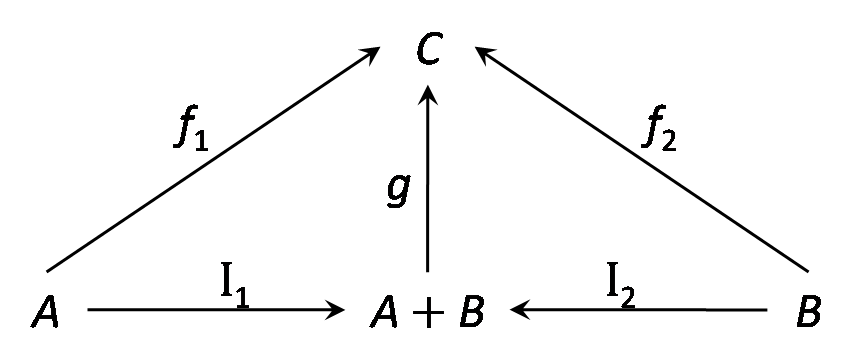
\includegraphics[scale=0.48]{./images/cat_cop}
\caption{Diagram of coproduct $ A+B $}
\label{figure:cat_cop}
\end{figure}

The coproducts in \textsc{Set} are the disjoint unions of sets. Let $ A $ and $ B $ be two sets. The disjoint union of them is defined by $ A+B = \{ \langle a,1 \rangle | a \in A \} \cup \{ \langle b,2 \rangle | b \in B \} $ with two injection functions $ \text{I}_1 : A \to A+B $ that takes all $ a $ in $ A $ to $ \langle a,1 \rangle $ in $ A+B $ and $ \text{I}_2 : B \to A+B $ that takes all $ b $ in $ B $ to $ \langle b,2 \rangle $ in $ A+B $. Given two functions $ f_1 : A \to C $ and $ f_2 : B \to C $, the function $ \langle f_1 , f_2 \rangle : A+B \to C $ is defined by $ \langle f_1 , f_2 \rangle ( \langle x,i \rangle ) = f_i (x) $ for all $ \langle x,i \rangle \in A+B $. Given any $ f_1 : A \to C $, $ f_2 : B \to C $ and $ g: A+B \to C $, the equations in definition \ref{definition:coproducts} are satisfied:
\begin{myitemize}
\item[i)] $ \langle f_1 | f_2 \rangle \circ \text{I}_i = f_i $\\
$
\begin{array}{ll}
  & ( \langle f_1 | f_2 \rangle \circ \text{I}_i )(x)\\
= & \langle f_1 | f_2 \rangle ( \text{I}_i (x))\\
= & \langle f_1 | f_2 \rangle ( \langle x,i \rangle )\\
= & f_i (x)
\end{array}
$\\
for any $ \langle x,i \rangle \in A+B $.
\item[ii)] $ \langle g \circ \text{I}_1 | g \circ \text{I}_2 \rangle = g $\\
$
\begin{array}{ll}
  & \langle g \circ \text{I}_1 | g \circ \text{I}_2 \rangle ( \langle x,i \rangle )\\
= & ( g \circ \text{I}_i )(x)\\
= & g( \text{I}_i (x) )\\
= & g( \langle x,i \rangle )
\end{array}
$\\
for any $ \langle x,i \rangle \in A+B $.
\end{myitemize}
\mbox\\
\\
One can form a set of functions which have the same domain and codomain. Similarly, the hom-set of morphisms may form an object. This idea brings our last basic construction, exponentials.

\begin{definition}[\textbf{Exponentials}]
\label{definition:exponentials}
Let $ \mathcal{C} $ be a category with products for all objects, and $ A $ and $ B $ be objects in $ \mathcal{C} $. The \emph{exponential}, also called \emph{function object}, of $ A $ and $ B $ is an object $ A \to B $ together with a morphism $ \text{App} : ( A \to B ) \times A \to B $, and for every object $ C $ in $ \mathcal{C} $, an operation $ \text{Curry} : \text{Hom}(C \times A,B) \to \text{Hom}(C, A \to B) $ such that for every $ h: C \times A \to B $ and $ k: C \to ( A \to B ) $, the following equations hold:
\begin{myitemize}
\item $ \text{App} \circ \langle \text{Curry} (h) \circ \text{Proj}_1 , \text{Proj}_2 \rangle = h $;
\item $ \text{Curry} ( \text{App} \circ \langle k \circ \text{Proj}_1 , \text{Proj}_2 \rangle ) = k $.
\end{myitemize}
\end{definition}

Using the definition of products of morphisms, $ f \times g = \langle f \circ \text{Proj}_1 , g \circ \text{Proj}_2 \rangle $, the two equations in definition \ref{definition:exponentials} can be rewritten as $ \text{App} \circ ( \text{Cutty}(h) \times \text{id} ) = h $ and $ \text{Curry}( \text{App} \circ (k \times \text{id})) = k $.

The commutative diagram representing the equations in the definition is shown in figure \ref{figure:cat_ex},where the morphism $ \text{Curry}(h): C \to (A \to B) $ is the unique $ k $.
\begin{figure}[h!]
\centering
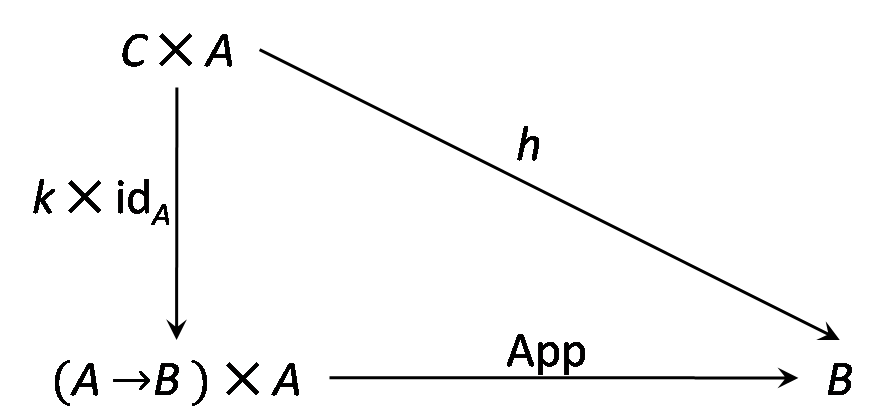
\includegraphics[scale=0.48]{./images/cat_ex}
\caption{Diagram of exponential $ A \to B $}
\label{figure:cat_ex}
\end{figure}

In \textsc{Set}, the exponent set $ A \to B $ of $ A $ and $ B $ is the set of functions from $ A $ to $ B $. The function $ \text{App} : (A \to B) \times A \to B $ is given by $ \text{App}( \langle f,a \rangle ) = f(a) $ for all $ f: A \to B $ and $ a \in A $. Given a function $ g: C \times A \to B $, the function $ \text{Curry}(g) $ is defined by $ ((\text{Curry}(g))(c))(a) = g( \langle c,a \rangle ) $ for all $ c \in C $ and $ a \in A $. Given any $ h: C \times A \to B $ and $ k: C \to (A \to B) $, the two equations in definition \ref{definition:exponentials} hold:
\begin{myitemize}
\item[i)] $ \text{App} \circ \langle \text{Curry} (h) \circ \text{Proj}_1 , \text{Proj}_2 \rangle = h $\\
$
\begin{array}{ll}
  & ( \text{App} \circ \langle \text{Curry} (h) \circ \text{Proj}_1 , \text{Proj}_2 \rangle )( \langle c,a \rangle )\\
= & \text{App}( \langle \text{Curry} (h) \circ \text{Proj}_1 , \text{Proj}_2 \rangle ( \langle c,a \rangle ) ) \\
= & \text{App}( \langle ( \text{Curry} (h) \circ \text{Proj}_1 ) ( \langle c,a \rangle ) , \text{Proj}_2 ( \langle c,a \rangle ) \rangle ) \\
= & \text{App}( \langle \text{Curry} (h) ( \text{Proj}_1 ( \langle c,a \rangle ) ), a \rangle ) \\
= & \text{App}( \langle ( \text{Curry} (h) )(c) , a \rangle ) \\
= & (( \text{Curry} (h) )(c))(a) \\
= & h( \langle c,a \rangle )
\end{array}
$\\
for any $ a \in A $ and $ c \in C $.
\item[ii)] $ \text{Curry} ( \text{App} \circ \langle k \circ \text{Proj}_1 , \text{Proj}_2 \rangle ) = k $\\
$
\begin{array}{ll}
  & (( \text{Curry} ( \text{App} \circ \langle k \circ \text{Proj}_1 , \text{Proj}_2 \rangle ))(c))(a)\\
= & ( \text{App} \circ \langle k \circ \text{Proj}_1 , \text{Proj}_2 \rangle )( \langle c,a \rangle ) \\
= & \text{App} ( \langle k \circ \text{Proj}_1 , \text{Proj}_2 \rangle ( \langle c,a \rangle ) ) \\
= & \text{App} ( \langle ( k \circ \text{Proj}_1 ) ( \langle c,a \rangle ) , \text{Proj}_2 ( \langle c,a \rangle ) \rangle ) \\
= & \text{App} ( \langle k ( \text{Proj}_1 ( \langle c,a \rangle ) ) , a \rangle ) \\
= & \text{App} ( \langle k (c) , a \rangle ) \\
= & (k(c))(a)
\end{array}
$\\
for any $ a \in A $ and $ c \in C $.
\end{myitemize}



%---------------------------------------------------------------------------%
%Cartesian Closed Categories
\subsubsection{Cartesian Closed Categories}
\label{sec:bg_cat_ccc}
Both products and exponentials have special importance for theories of computation. A two-argument function can be reduced to a one-argument function yielding a function from the second argument to the result. This passage is called \emph{currying}. And exponentials give a categorical interpretation to the notion of currying. Therefore, categories with products and exponentials for every pair of objects are important enough to deserve a special name.

\begin{definition}[\textbf{Cartesian Closed Categories}]
\label{definition:ccc}
A category $ \mathcal{C} $ is \emph{cartesian closed} iff
\begin{myitemize}
\item it contains a terminal object $ unit $;
\item for every pair of objects $ A $ and $ B $ in $ \mathcal{C} $, there is a product;
\item for every pair of objects $ A $ and $ B $ in $ \mathcal{C} $, there is an exponential.
\end{myitemize}
\end{definition}

\begin{proposition}
\label{proposition:eqns}
The following identities hold in every cartesian closed category:
\begin{myitemize}
\item[(1)] $ \langle f,g \rangle \circ h = \langle f \circ h , g \circ h \rangle $\\
where $ f: C \to A $, $ g: C \to B $ and $ h: D \to C $;
\item[(2)] $ \langle f,g \rangle = ( f \times \text{id}_B ) \circ \langle \text{id}_C , g \rangle $\\
where $ f: C \to A $ and $ g: C \to B $;
\item[(3)] $ \text{Curry}(f) \circ h = \text{Curry}(f \circ (h \times \text{id})) $\\
where $ f: A \times B \to C $ and $ h: D \to A $.
\end{myitemize}
\end{proposition}

\begin{proof}
These three equations have been proved by the diagrams in figures \ref{figure:cat_eqn1}, \ref{figure:cat_eqn2} , and \ref{figure:cat_eqn3}. But they can also be proved by using the equations given in definition \ref{definition:products} and \ref{definition:exponentials} .

\begin{figure}[h!]
\centering
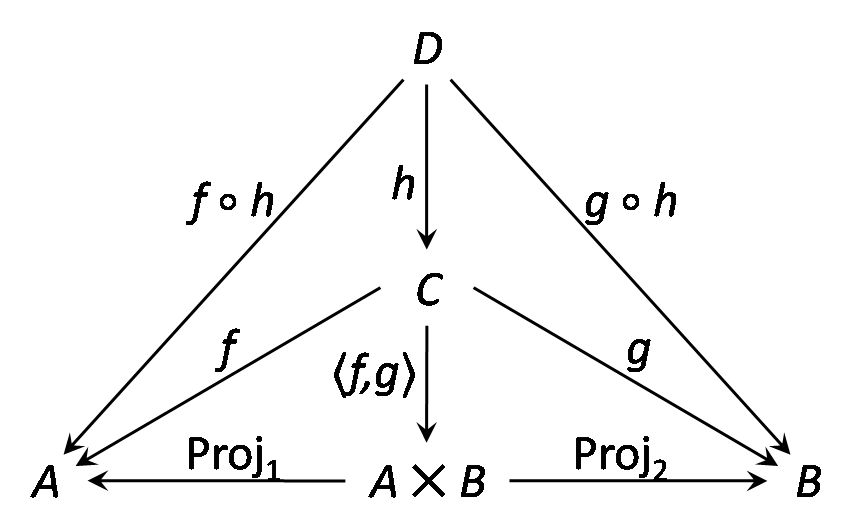
\includegraphics[scale=0.48]{./images/cat_eqn1}
\caption{Diagram of $ \langle f,g \rangle \circ h = \langle f \circ h , g \circ h \rangle $}
\label{figure:cat_eqn1}
\end{figure}
\begin{figure}[h!]
\centering
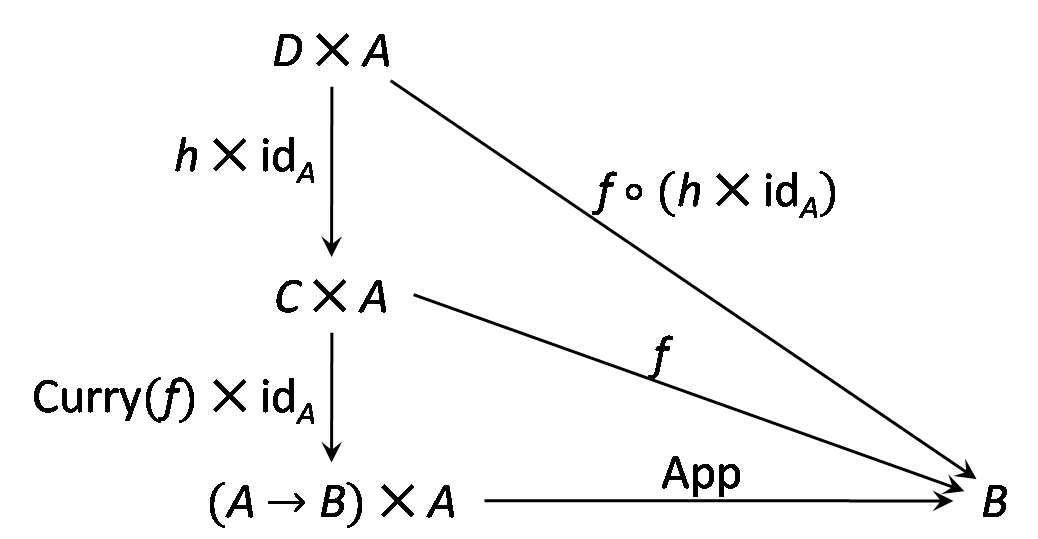
\includegraphics[scale=0.48]{./images/cat_eqn2}
\caption{Diagram of $ \langle f,g \rangle = ( f \times \text{id}_B ) \circ \langle \text{id}_C , g \rangle $}
\label{figure:cat_eqn2}
\end{figure}
\begin{figure}[h!]
\centering
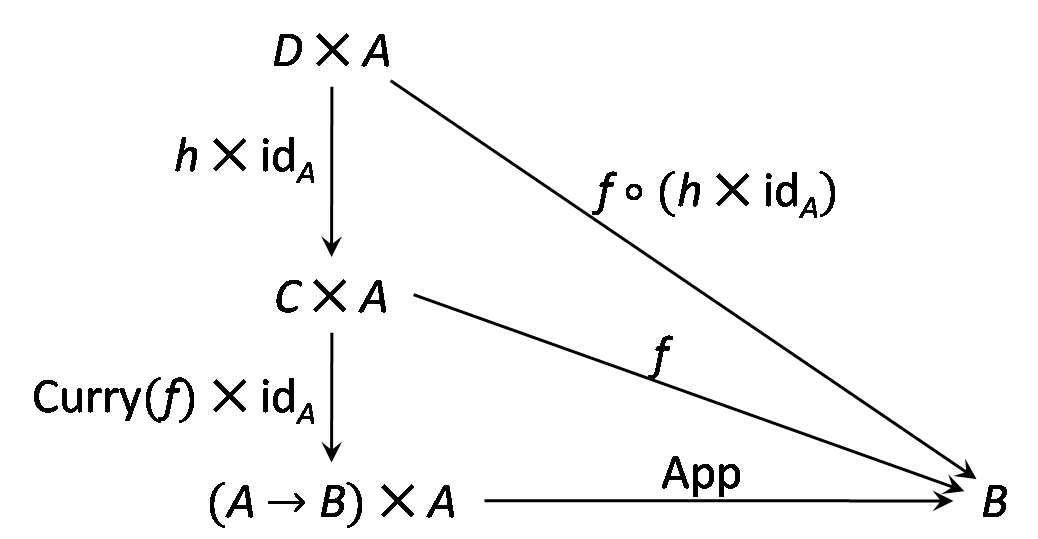
\includegraphics[scale=0.48]{./images/cat_eqn3}
\caption{Diagram of $ \text{Curry}(f) \circ h = \text{Curry}(f \circ (h \times \text{id})) $}
\label{figure:cat_eqn3}
\end{figure}

\begin{myitemize}
\item[(1)] $ \text{Proj}_1 \circ ( \langle f,g \rangle \circ h ) = ( \text{Proj}_1 \circ \langle f,g \rangle ) \circ h = f \circ h $\\
$ \text{Proj}_2 \circ ( \langle f,g \rangle \circ h ) = ( \text{Proj}_2 \circ \langle f,g \rangle ) \circ h = g \circ h $\\
$ \langle \text{Proj}_1 \circ ( \langle f,g \rangle \circ h ) , \text{Proj}_2 \circ ( \langle f,g \rangle \circ h ) \rangle = \langle f \circ h , g \circ h \rangle $\\
Since we have $ \langle \text{Proj}_1 \circ g , \text{Proj}_2 \circ g \rangle = g $ (in definition \ref{definition:products}), then $ \langle f,g \rangle \circ h = \langle f \circ h , g \circ h \rangle $ holds.
\item[(2)] $ f \times \text{id}_B = \langle f \circ \text{Proj}_1 , \text{id}_B \circ \text{Proj}_2 \rangle $ (by the definition of products of morphisms) \\
$
\begin{array}{ll}
  & ( f \times \text{id}_B ) \circ \langle \text{id}_C , g \rangle \\
= & \langle f \circ \text{Proj}_1 , \text{id}_B \circ \text{Proj}_2 \rangle \circ \langle \text{id}_C , g \rangle \\
= & \langle f \circ \text{Proj}_1 , \text{Proj}_2 \rangle \circ \langle \text{id}_C , g \rangle \\
  & (\text{by } \langle f,g \rangle \circ h = \langle f \circ h , g \circ h \rangle \text{ in (1) } ) \\ 
= & \langle f \circ \text{Proj}_1 \circ \langle \text{id}_C , g \rangle , \text{Proj}_2 \circ \langle \text{id}_C , g \rangle \rangle \\
  & (\text{by } \text{Proj}_i \circ \langle f_1,f_2 \rangle = f_i ) \\
= & \langle f \circ \text{id}_C , g \rangle \\
= & \langle f, g \rangle \\
\end{array}
$
\item[(3)] $ f = \text{App} \circ ( \text{Curry}(f) \times \text{id})) $ (by $ \text{App} \circ ( \text{Cutty}(h) \times \text{id} ) = h $ in definition \ref{definition:exponentials})\\
$
\begin{array}{ll}
  & \text{Curry}(f \circ (h \times \text{id})) \\
= & \text{Curry}(( \text{App} \circ ( \text{Curry}(f) \times \text{id})) ) \circ (h \times \text{id})) \\
= & \text{Curry}( \text{App} \circ (( \text{Curry}(f) \times \text{id})) \circ (h \times \text{id}))) \\
  & (\text{by proposition } \ref{proposition:pro_of_mor} \text{ } ( g_1 \times g_2 ) \circ ( f_1 \times f_2 ) = ( g_1 \circ f_1 ) \times ( g_2 \circ f_2 ) ) \\
= & \text{Curry}( \text{App} \circ (( \text{Curry}(f) \circ h ) \times ( \text{id} \circ \text{id} ))) \\
= & \text{Curry}( \text{App} \circ (( \text{Curry}(f) \circ h ) \times \text{id} ))) \\
  & (\text{by } \text{Curry}( \text{App} \circ (k \times \text{id})) = k \text{ in definition } \ref{definition:exponentials} ) \\
= & \text{Curry}(f) \circ h
\end{array}
$
\end{myitemize}
\end{proof}

The following gives some examples and one non-example of CCCs.
\begin{myitemize}
\item[(1)] \textsc{Set}\\
\textsc{Set} has been already given as an example of each categorical construction. It is cartesian closed since it satisfies the three conditions:
  \begin{myitemize}
  \item Any singleton set can be the terminal object (it does not matter which one it exactly is since all the singleton sets are isomorphic);
  \item The product of sets $ A $ and $ B $ is the cartesian product of $ A $ and $ B $;
  \item The exponential of sets $ A $ and $ B $ is the set of functions from $ A $ to $ B $.
  \end{myitemize}
  
\item[(2)] \textsc{Pos}\\
\textsc{Pos} is the category whose objects are posets and whose morphisms are monotone maps. The identity of object $ \mathcal{A} = (A,\leq _A) $ in \textsc{Pos} is the identity map $ \text{id}_A: A \to A $ such that $ \text{id}_A(a) = a $ for all $ a \in A $. The composition of morphisms is the composition of maps. Both identity and composition still preserve the monotonicity property.\\
\textsc{Pos} is cartesian closed:
  \begin{myitemize}
  \item Any singleton poset can be the terminal object $ unit $. Then the map $ \text{One}^A: A \to unit $ from any poset $ \mathcal{A} $ to this singleton poset is unique.
  \item The product $ \mathcal{A} \times \mathcal{B} = (A \times B, \leq_{A \times B}) $ of posets $ \mathcal{A} = (A,\leq _A) $ and $ \mathcal{B} = (B,\leq _B) $ is the cartesian product of sets $ A $ and $ B $ with the ordering $ \leq_{A \times B} $ which is defined by $ \langle a,b \rangle \leq_{A \times B} \langle a',b' \rangle $ iff $ a \leq_A a' $ and $ b \leq_B b' $.\\
  The projections are the coordinate functions $ \text{Proj}_1 : A \times B \to A $ and $ \text{Proj}_2 : A \times B \to B $ which just return one of the two components in the pair. So they preserve the monotonicity.\\
  Given two monotone maps $ f_1: A \to B $ and $ f_2: A \to C $, the map $ \langle f_1, f_2 \rangle : A \to B \times C $ is defined by $ \langle f_1, f_2 \rangle (a) = \langle f_1(a), f_2(a) \rangle $ for all $ a \in A $. Suppose $ a,a' \in A $ and $ a \leq_A a' $, then $ f_1(a) \leq_B f_1(a') $ and $ f_2(a) \leq_C f_2(a') $. According to the above definition, we have $ \langle f_1, f_2 \rangle (a) \leq_{B \times C} \langle f_1, f_2 \rangle (a') $. Hence, the map $ \langle f_1, f_2 \rangle $ is monotone.\\
  In the same way as \textsc{Set}, \textsc{Pos} satisfies the equations in definition \ref{definition:products}.
  \item The exponential $ \mathcal{A} \to \mathcal{B} = (A \to B, \leq_{A \to B}) $ of posets $ \mathcal{A} = (A,\leq _A) $ and $ \mathcal{B} = (B,\leq _B) $ is the set of monotone maps from $ A $ to $ B $ and a ordering $ \leq_{A \to B} $ defined by, given $ f, f' : A \to B $, $ f \leq_{A \to B} f' $ iff $ f(a) \leq_B f'(a) $ for all $ a \in A $.\\
  Given a monotone map $ g: A \times B \to C $, the map $ \text{Curry}(g): A \to (B \to C) $ is defined by $ ((\text{Curry}(g))(a))(b) = g( \langle a,b \rangle ) $ for all $ a \in A $ and $ b \in B $. Suppose $ a,a' \in A $, $ b \in B $ and $ a \leq_A a' $, we have $ (\text{Curry}(g))(a) \leq_{B \to C} (\text{Curry}(g))(a') $ because $ ((\text{Curry}(g))(a))(b) = g( \langle a,b \rangle ) \leq_C g( \langle a',b \rangle ) = ((\text{Curry}(g))(a'))(b) $ for any $ b \in B $; therefore, \text{Curry}(g) is monotone.\\
  The map $ \text{App} : (B \to C) \times B \to C $ is defined by $ \text{App}( \langle h,b \rangle ) = h(b) $ for all $ h: B \to C $ and $ b \in B $. Suppose $ h,h': B \to C $ and $ b.b' \in B $ with $ h \leq_{B \to C} h' $ and $ b \leq_B b' $, we have $ \langle h,b \rangle \leq_{(B \to C) \times B} \langle h',b' \rangle $ by the definition of $ \leq_{(B \to C) \times B} $ and then $ \text{App}( \langle h,b \rangle ) = h(b) \leq_C h(b') \leq_C h'(b') = \text{App}( \langle h',b' \rangle ) $; therefore, $ \text{App} $ is also monotone.\\
  \textsc{Pos} also satisfies the equations in definition \ref{definition:exponentials}. The proof is carried out in the same way of \textsc{Set}.
  \end{myitemize}
  
\item[(3)] \textsc{Pos}$_\bot$\\
\textsc{Pos}$_\bot$ is the  same as the category \textsc{Pos} except that each poset has a least element $ \bot $. We construct its identity, composition, terminal object, products, and exponentials in the same way of \textsc{Pos}.\\
However, the least elements in products and exponentials should be defined particularly. If $ \bot _A $ and $ \bot _B $ are least elements in posets $ \mathcal{A} $ and $ \mathcal{B} $, the least element in product $ \mathcal{A} \times \mathcal{B} $ is $ \bot _{A \times B} = \langle \bot _A , \bot _B \rangle $. The least element $ \bot _{A \to B} $ in exponential $ \mathcal{A} \to \mathcal{B} $ is the map converting any $ a \in A $ to $ \bot _B $, i.e. $ \bot _{A \to B} (a) = \bot _B $ for all $ a \in A $.\\
Since the definition of morphisms in \textsc{Pos}$_\bot$ is still the same as the one in \textsc{Pos}, \textsc{Pos}$_\bot$ should be cartesian closed.

\item[(4)] \textsc{Pos}$_{\bot !}$ \\
In category \textsc{Pos}$_{\bot !}$, the objects are posets with least elements and the morphisms are monotone maps that preserve the least element $ \bot $, i.e. for every monotone map $ f: A \to B $, $ f( \bot _A ) = \bot _B $.

Though it looks similar to \textsc{Pos}$_\bot$, \textsc{Pos}$_{\bot !}$ is not cartesian closed. If we still define the products and exponentials in the same way as \textsc{Pos}, we we find that it cannot satisfy all the three conditions of cartesian closed categories:
\begin{myitemize}
\item Any singleton poset is still a terminal object in \textsc{Pos}$_{\bot !}$.
\item The cartesian products can work as products in \textsc{Pos}$_{\bot !}$. For any $ f_1: A \to B $ and $ f_2: A \to C $, the map $ \langle f_1, f_2 \rangle $ has been proven to be monotone in (2). According to the definition of $ \langle \cdot, \cdot \rangle $, $ \langle f_1, f_2 \rangle (\bot_A) = \langle f_1(\bot_A), f_2(\bot_A) \rangle = \langle \bot_B, \bot_C \rangle = \bot_{B \times C} $. It preserves $ \bot $; therefore, the cartesian products are products in in \textsc{Pos}$_{\bot !}$.
\item The exponentials defined in (2) are not exponentials in \textsc{Pos}$_{\bot !}$. Assume \textsc{Pos}$_{\bot !}$ has the same exponentials as \textsc{Pos}, then for any morphism $ f: A \times B \to C $ there should be a unique $ g = \text{Curry}(f): A \to (B \to C) $ which is isomorphic to $ f $. Since $ g(\bot _A)= \bot _{B \to C} $ and $ \bot _{B \to C} (b) = \bot _C $ for any $ b \in B $, we have $ (g(\bot _A))(b) = \bot _C $. However, $ f $ may not map all $ \langle \bot _A , b \rangle $ to $ \bot _C $, which means that $ f \ncong g $. So the exponentials in \textsc{Pos} are not exponentials in \textsc{Pos}$_{\bot !}$.
\end{myitemize}
One may still think that \textsc{Pos}$_{\bot !}$ is cartesian closed because we may be able to find other products or exponentials for it.\\
If we construct a ``product'' of $ A $ and $ B $ by
\begin{center}
$ A \bigotimes B = \{ \langle a,b \rangle | a \in A - \{ \bot_A \}, b \in B -\{ \bot_B \} \} \cup \{ \langle \bot_A, \bot_B \rangle \} $,
\end{center}
then the exponentials from \textsc{Pos} work in \textsc{Pos}$_{\bot !}$ now since $ \langle \bot_A,b \rangle $ is not an element in ``product'' $ A \bigotimes B $. However, this $ \bigotimes $ is not a categorical product. Given any $ f_1: A \to B $ and $ f_2: A \to C $, the map $ \langle f_1, f_2 \rangle $ should map all $ a \in A $ to elements in $ B \bigotimes C $. But $ \langle \bot_{A \to B}, f_2 \rangle (a) = \langle \bot_{A \to B}(a), f_2(a) \rangle = \langle \bot_B, f_2(a) \rangle $ and $ \langle \bot_B, f_2(a) \rangle \not\in B \bigotimes C $ if $ f_2(a) \neq \bot_C $.\\
The fact is that \textsc{Pos}$_{\bot !}$ does not have exponentials. Let $ unit $ be the terminal object in \textsc{Pos}$_{\bot !}$. We know that for any object $ A $, $ unit \times A \cong A $. Then their hom-sets should be isomorphic as well, i.e. $ \text{Hom}(A,A) \cong \text{Hom}(unit \times A,A) $. Provided that \textsc{Pos}$_{\bot !}$ has exponentials, we have $ \text{Hom}(unit \times A,A) \cong \text{Hom}(unit, A \to A) $ and so $ \text{Hom}(A,A) \cong \text{Hom}(unit, A \to A) $. If $ A $ is not singleton (terminal object), then there can be many monotone maps from $ A $ to $ A $, which means $ \text{Hom}(A,A) $ can have many elements. However, $ \text{Hom}(unit, A \to A) $ has only one morphism since there is only one map from the singleton poset to any other poset. $ \text{Hom}(A,A) $ is not isomorphic to  $ \text{Hom}(unit, A \to A) $; therefore, \textsc{Pos}$_{\bot !}$ cannot have exponentials.

\end{myitemize}